% !Mode:: "TeX:UTF-8"

\documentclass[literaturereview]{zjutreport}
\graphicspath{{figures/}}  % 定义所有的eps文件在 figures 子目录下

\begin{document}           % 开始全文

%论文题目:{中文}
\zjuttitle{基于内存数据库的大数据应用系统的设计与实现}
%作者:{中文姓名}{学号}
\zjutauthor{陈佳鹏}{200926630503}
%指导教师:{导师中文名}
\zjutmentor{陈~~~~波}
%个人信息:{毕业年份}{专业名称}
\zjutinfo{2013}{软件工程}
%学院信息:{学院中文}
\zjutcollege{计算机科学与技术学院}
%日期:{提交日期}
\zjutdate{2013年03月}

% !Mode:: "TeX:UTF-8"
%%============================================================
%% 中文封面
\thispagestyle{empty}
\pdfbookmark[-1]{\zjuttitlec}{zjutreportcover}
\phantomsection \label{zjutreportcover}
\vspace*{-2.5mm}
% 校名
\begin{center}
   
\includegraphics[width=98.40mm]{figures/zjut}
\end{center}
\vspace*{9.66mm}
\centerline{\songti\yihao{\reporttitle}}
\vspace*{10.0mm}
\centerline{\heiti\xiaoer\textbf{(\zjutgrade\ 届)}}
\vspace*{8.5mm}
% 校徽
\begin{center}
  
\includegraphics[width=27.3mm]{figures/zjutlogo}
\end{center}

\vspace*{0.0mm}
\renewcommand{\arraystretch}{1.0}
\hspace*{7.4mm}
{\songti\erhao{论文题目}}
\hspace{6mm}
\begin{minipage}[t]{95mm}
    \linespread{1.1}{\songti\xiaoer\uline{\zjuttitlec}}
\end{minipage}
\vspace*{9mm}
\begin{center}
    \setlength{\arrayrulewidth}{0.5pt}
    {\songti\sihao
        \renewcommand{\arraystretch}{1.4}
        \begin{tabular}{lc}
            作者姓名 \qquad &  \zjutauthornamec \\ \cline{2-2}
            指导教师\qquad &  \zjutmentorc\\ \cline{2-2}
            \\
            学科(专业)\qquad &  \zjutmajor \\ \cline{2-2}
            所在学院\qquad &  \zjutcollegec \\ \cline{2-2}\cline{2-2}
            提交日期\qquad & \zjutsubmitteddatee \\ \cline{2-2}
        \end{tabular}
    }
\end{center}

      % 封面

\frontmatter

\pagenumbering{Roman}
\begingroup % 在组内的chapter不换行
\let\clearpage\relax % chapter之后不换页

%%%%%%%%%% 标题 %%%%%%%%%%
\titleformat{\chapter}[block]{\sihao\heiti\filcenter\bfseries}{\CJKnumber{\thechapter}}{1ex}{}{} % 标题居中,黑体三号
\chapter*{基于内存数据库的大数据应用系统的设计与实现}
\titleformat{\chapter}[block]{\xiaosi\heiti}{\CJKnumber{\thechapter}、}{1ex}{}{} % 恢复标题居左,黑体四号

%%%%%%%%%% 摘要 %%%%%%%%%%
% !Mode:: "TeX:UTF-8"

%%%%% 摘要 %%%%%
\abstractc{本文是基于内存数据库的大数据应用系统的设计与实现的一篇文献综述,先介绍项目的由来及其研究意思,然后介绍项目的国内外研究现状及难点以定位项目开发的一个大环境,明确当前同类项目的研究情况。接着本文简述内存数据库系统的结构,紧接着介绍系统开发中所需的关键技术。}

%%%%% 关键词 %%%%%
\keywordsc{内存数据库,索引结构,并发控制,T树,数据恢复,影子内存,混合日志}
     % 中文摘要

%%%%%%%%%% 正文 %%%%%%%%%%
\mainmatter
% \makeatletter
\chapter{引言}
在当今的信息化建设过程中,数据库在维护和管理数据这一方面扮演了非常重要
的角色。信息化改造成功与否的关键往往在于是否有一个合适的数据库系统。传统的磁盘数据
库(Disk Resident Database,DRDB)经过几十年的发展,由于功能完备,稳定
性好,因而常用于银行,电信等公司,用于进行管理客户资料,管理部门档案
等日常应用,且一直有着令人满意的表现。但是随着科技的发展,
一批新兴行业大量涌现,比如工业控制,航空航天,数据通信,电力调度,证券
交易等,这些新产业所要求的数据库系统通常并不需要强大而完备的功能和复杂的事物处理能力,
而是要能在指定的时刻或时间内对大量的数据进行采集,处理并能正确的响应的高速
性能。此时,DRDB不能很好地支持实时性,不能满足实时性要求,主
要原因是DRDB的事务涉及I/O操作、缓冲区管理和页违例等事
件,导致执行时间的不可预知性和弱实时性,使得事务的实时性和预测性较差[17]。

对DRDB而言,由于磁盘存取、内外存数据的传递、缓冲区管理、排队等待及锁延迟等使得事务
实际平均执行时间和预计估算的最坏情况相差甚大。但是,如果将整个数据库或其“热”数据全部放入内存
,使每个事务在执行过程中没有I/O损耗,这样一来,系统能较准确的估算和安排事务的运行时间,
使之具有较好的动态可预报性。这就是内存数据库(Main Memory Databse,MMDB)出现的原因。

MMDB与DRDB两者之间最主要的差别在于主版本数据的存放位置不同,前者在内存,后
者在磁盘。由于内存与磁盘在访问速度、易失性、访问模式等方面存在很大
的差异[16]。如表~\ref{tab:table1}~所示。

\begin{table}[htbp]
\caption{MMDB和DRDB的差别}\label{tab:table1}
\vspace{0.5em}{\wuhao
\begin{tabularx}{\textwidth}{lXX}
\toprule[1.5pt]
性能 & MMDB & DRDB\\
\midrule[1pt]
数据存储 & 行、列级和段分区式储存模型,模型在内存中不一定连续存放 & Sybase~IQ采用列级储存,其他数据库系统采用行级存储,在磁盘上连续存放\\
缓冲管理 & 不需要 & 需要\\
并发控制 & 采用封锁机制、多版本等方式,一般用较大粒度的锁,如库级锁、表级锁或采用乐观封锁机制 & 采用封锁机制、时间戳、多版本等方式,为了提高事务的并发度,一般支持多粒度和多种类型的锁\\
恢复机制 & 备份、日志和检查点技术,采用预提交、组提交等提交方式;用稳定内存来存储日志记录 & 采用备份、日志、检查点、保存点等技术\\
索引结构 & T树、hash & B树、hash\\
查询优化 & 基于CPU以及cache代价 & 基于I/O代价\\

\bottomrule[1.5pt]
\end{tabularx}}
\vspace{\baselineskip}
\end{table}

\chapter{研究意义}
数据库技术在几十年的发展中,功能逐渐完善,现在主流的数据库软件动辄支持
上TB的数据容量,而且经过各种技术革新后,能支持大业务并发操作。但一般的
数据库软件,数据都无一例外的存储于磁盘,数据库软件在需要使用到某份数据
时,通过操作系统调用,从磁盘读取出来,读入到内存中,进行运算、比较或其
他文本型操作,从而实现业务需求。磁盘是当前主流数据库的主要瓶颈所在。一
般硬盘的读取速度为毫秒级时采用光纤盘阵,并部署成RAID机制,如读写速度更
快的RAID0,但仍然逃脱不出毫秒级的范畴。

磁盘技术即使不断革新,到现在出现的SSD(Solid State Disk)技术,但对要求
极其苛刻的大型数据库而言,仍然是杯水车薪。测试结果表明,SSD技术在随机读
写方面的性能,比普通硬盘提升了约5倍。而且SSD技术目前不是特别完善,还存
在硬盘容量小,价格过于昂贵等致命伤。

所以内存数据库是高响应要求数据库系统的最佳、甚至唯一选择。现在,不仅仅
电信级数据库,甚至包括大型互联网数据库,也要求业务操作的响应时间为毫秒
级。这对数据库的响应速度提出了很苛刻的要求。唯一的途径就是,将数据缓存
在内存里。让应用程序直接从内存里读写数据,规避硬盘读写,从而极大的提高
数据库对外性能。

\chapter{研究现状}
MMDB的研究始于上个世纪80年代,经过了20多年的发展,研究者们已对其相关的
体系结构,数据组织,事务处理,并发控制和备份恢复等相关技术进行了大量研
究和探讨,同时针对硬件,软件和算法设计提出了许多不同的策略和实现方案。
目前对MMDB的研究主要集中在以下方面:

1. 体系结构:包括系统的体系结构和存储体
系结构两部分内容,前者侧重于研究多处理器在MMDB中的应用,
而后者则侧重于研究非易失性内存(Non-Volatile Memory,NVM)在MMDB中
的应用。

2. 事务处理:主要对事务的提交和日志记录、查询优化,
(尤其是联机查询的优化)进行大量的研究。如开发了“提前提交”等策略以优化事务的初始如对事
务的初始处理、提交处理、并发控制、完整性和安全性检验等,加速并发事务的
响应时间,查询的优化主要在于对减少查询中中间关系的算法的研究。

3. 数据组织与存取方法,这方面主要针对MMDB存储介质的特性设计了许多适合内
存特性的数据存储组织结构和存取方式,索引结构和存储策略,MMDB的压缩,如
AVL树索引结构,区段式组织结构,位图分配法等,Hash结构[19]。

4. MMDB的备份和恢复,备份方面更是提出了多种方案,为了预防MMDB的崩溃主要
是结合检查点和日志来保证MMDB(MMDB)在崩溃后的可恢复性,提出了许多具体
的算法如FUZZY(模糊)检验点策略,BLACK/WHITE(黑/白)策略,COPY-ON-UPDATE
(变更拷贝)检验点等,同时研究了非易失性内存在MMDB备份中的应用,如“影子
内存”技术等。而备份恢复方面则是对MMDB重启之后的装入策略的研究,结合内存
数据中数据使用的频率和优先级提出一种最优的装入策略,目前提出了“部分重装”
等策略,MMDB的目录恢复后就启动系统,然后根据要求再继续重装,从而提高CPU
的使用率和事务的吞吐量。

5. MMDB的并发控制,在短小事务时,往往采用大力度的锁,MMDB近似于串行处理,
串行化执行事务一方面使得并发控制的代价几乎完全消除,同时也能减少CPU的cache
缓存和虚拟内存页表TLB的刷新频率;而对于长事务和多处理机环境串行处理明显
不合适,这样就必需应用而合适的锁机制来支持并发操作,目前提出了二级层次封
锁协议方案、乐观并发控制方法、使用可扩展的哈希技术的方法等。

近些年来随着大容量廉价的内存投入市场,使得上诉的各种技术也逐渐在内存数
据库的设计和实现上得到了应用,内存数据库也不在停留在理论研究阶段,内存
数据库走向了实际应用阶段,各高校和研究机构发布了研究模型系统,一些公司
也推出了用于工业的商用内存数据库系统。目前工业应用上比较流行的商用系统
有Amazon的Dynamo[1],SAP的Hana[8],Oracle公司的内存数据库Berkeley DB,内存数据库SQLite,开源的内存数据库
FastDB,以及McObject公司的eXtremDB。他们的特点如表~\ref{tab:table2}~所示:

\begin{table}[htbp]
\caption{主流内存数据库}\label{tab:table2}
\vspace{0.5em}{\wuhao
\begin{tabularx}{\textwidth}{llX}
\toprule[1.5pt]
内存数据库名 & 厂商 & 特点\\
\midrule[1pt]
Berkeley DB & Oracle & Berkeley DB数据库系统简单、小巧、可靠、高性能,
提供了一系列应用程序接口(API),应用程序和Berkeley DB 所提供的库在一起编译成为可执行程序。每一个记录由关键字和数据(KEY/VALUE)组成的键值对构成\\
SQLite & 开源 & SQLite是一款轻型的数据库,它的设计目标是针对嵌入式系统,提供了很多语言的接口,支持SQL语句,支持事务处理,它占用资源非常的低,支持跨平台操作,操作使用简单。每完成一次操作需要进行内存和磁盘之间的同步\\
ExtremeDB & McObject & ExtremDB是为实时系统及嵌入式系统而特别设计的,完全工作在主内存中,不基于文件系统,支持事务,支持部分SQL,支持稳定的RAM。通过数据库定义语言为应用系统各自的API。具有工业应用强度\\
FastDB & 开源 & FastDB是一个高效率的内存数据库系统,支持事务、在线备份和系统崩溃之后的自动恢复,支持类似SQL语言并提供了C++接口,算法和结构的优化都是基于数据存放在内存中这个假设上,但物理内存较小时也可使用\\
\bottomrule[1.5pt]
\end{tabularx}}
\vspace{\baselineskip}
\end{table}

\chapter{系统实现技术方法研究}
\section{内存数据的组织结构}
在MMDB系统设计时,广泛使用了现代操作系统提供的共享内存机制,系统初始化
时将整个数据库装入一片共享内存区,运行时,应用进程可以把整个数据库或一
部分映射到自己的虚地址空间进行直接访问。针对关系和索引数据全在内存中这
一特点,指针在数据结构和数据访问中被广泛的使用。应用进程可以通过指针,
也可以通过位置独立的数据库偏移量访问数据,无需像DRDB那样与缓冲区管理器
交互。另外,由于指针长度固定,因此变长字段问题可以很好解决。其次,若一
个大的数据对象在数据库中多次出现,则内存中只需存储一次,其它地方使用指
针来引用。

MMDB中关系的存储通常采用分级结构,同时强调元数据与数据应分区组织,以提
高安全性。在Starburst[16]中,存储结构分两层:段(Segment)和分区(Partition)
。段是可变长的,一个段由多个固定长的分区组成,每个段存放一个关系,但并
不要求构成一个段的分区空间上连续。分区则是Starburst的基本内存分配回收单
元,其长度固定。分区的结构由两部分组成,其中Free space存放记录插槽
(Record dot),Heap space存放分区控制信息和记录(即元组)本身。
整个数据库维护一个段表,段表中的每一项是一个段控制块。段控制块中包含一
个分区表、段latch、和索引链表的头指针。图~\ref{fig:starburst}~描述了
Starburst的内存数据组织结构图。

\begin{figure}[htbp]
%%% TODO Starburst from 内存数据库技术综述.pdf%%%
\centering
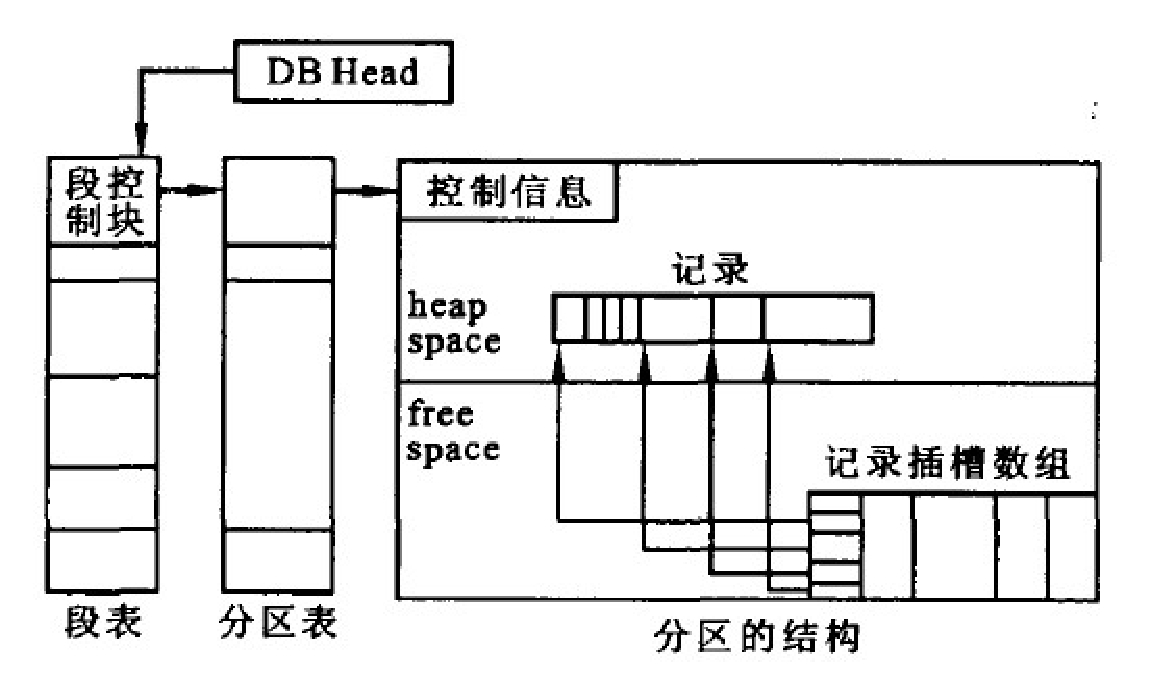
\includegraphics[width=0.4\textwidth]{starburst}
\caption{Starburst内部结构}\label{fig:starburst}
\vspace{\baselineskip}
\end{figure}

从图2中可以看到:一条记录本身放在分区的Heap区,对记录的访问是通过放在
Free区的记录插槽进行的。记录插槽中包含一个指向相应记录各字段在Heap中
地址的指针数组,由于指针的长度都一样,因此记录中不等长字段问题可以通
过包含字段指针数组的等长记录插槽解决;同时,在关系创建后,若增加关系
的字段,则可以通过在记录插槽预留的Tail结构进行扩展,所需空间在分区的
Heap中分配。当一个事务要访问记录时,先根据关键字查索引,找到该记录的
RID。一个RID是一个由段号、分区号、和记录插槽在分区中的偏移量组成的三
元组,用RID可以很快找到记录插槽,从而最终定位一条记录。

\section{索引技术}
\subsection{T树}
DRDB采用的索引结构主要是B/B$+$树,其设计目标是减少访问磁盘数据的IO次
数。而在MMDB中,通常采用了一种新的索引结构T树,其设计目标是减少内存开
销和CPU指令数。T树[16]是由AVL树和B树发展而来,它是一种一个节点包含多个元
素的二叉树,如图~\ref{fig:treenode}~所示。

\begin{figure}[htbp]
%%% TODO 插入T树node图  from 内存数据库关键技术研究.pdf%%%
\centering
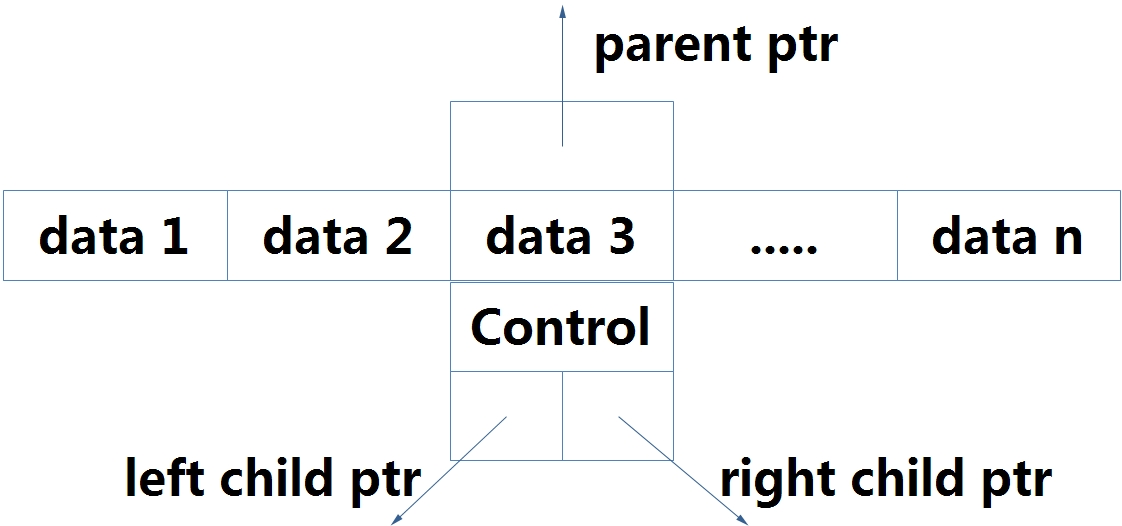
\includegraphics[width=0.4\textwidth]{treenode}
\caption{T树节点}\label{fig:treenode}
\vspace{\baselineskip}
\end{figure}

由于是二叉树,T树保持了AVL树二分查找的高效率,同时一个T节点包含多个
元素,像B树一样,每个节点的充满程度保持在半满和全满之间,这样索引一
般不再需要溢出块,由插入和删除所引起的数据移动通常只需在一个节点内
进行,减少了为保持树的平衡所必须进行的旋转操作,因此T树又保持了B树
优异的更新和存储特性。由于索引和数据全在内存中,在一个T树节点中不需
要像B树那样存放N个索引键值一指针对,只需存放指向内存中相应记录对应
字段的指针,这样索引中变长字段的存储不再是问题,另外,由于指针一般
比它指向的字段要小,大量的空间也被节省了。

\subsection{Hashing}
为了快速地定位数据库的记录,内存数据库中广泛使用的哈希索引有链接桶
哈希(chained bucket hashing)、可扩展哈希(extendible hashing)、
线性哈希(linear hashing)、修正的线性哈希(modified linear hashing)
,其中链接桶的哈希使用静态结构处理冲突,速度很快,但不适合动态环境。
基于等值的比较,哈希技术能够快速地访问数据库,且易于实现,但不支持
范围检索。

\section{并发控制}
内存数据库中使用的并发控制与磁盘数据库中的并发控制基本相同,细节上
存在一定差异。Starburst系统[16]使用封锁机制来保证事务的ACID特性。
Starburst系统中有两个粒度的锁:表级锁和记录级锁。其封
锁机制具有以下两个方面的特点:1)锁信息直接与表和记录
本身关联,不需要哈希表来存放锁信息,可消除通过哈希表查
找定位锁信息的开销;2)使用动态锁机制来维护表的锁粒度
级别。Starburst根据系统对关系的共享程度的需求,动态地
改变每个关系的锁粒度。因为表级锁比记录级锁开销小,因
此当不需要较细的锁粒度时推荐表级锁。如果当一个或者多
个事务在访问表时被其他事务阻塞,表级锁被分解成为记录
级锁。当不再需要细粒度锁时,记录级锁被转化为表级锁。

对于传统内存数据库,数据存储在内存中,事务执行时间较短,持锁时间也较
短,封锁产生的CPU代价会对性能产生严重的影响,系统中冲突较少,所以可
以采用以下方法减少锁的开销:

1)采用较大的锁粒度(如表级锁),因为数据常驻内存后,对数据的竞争已
很低,细粒度锁的优点对改善性能的意义已不大

2)采用乐观加锁方式

3)减少锁的类型

4)将锁信息存储在数据本身

\section{恢复机制}
将日志写在何处以及何时将日志写人磁盘在内存数据库中是一个非常重要的
问题。一些研究者提出了预提交、组提交等方法来降低日志I/O的代价,并
且提出使用稳定内存存储日志的方法:首先将日志存储在稳定内存中,然后
提交事务,再异步地把日志写入磁盘。在MMDB中,只有在事务提交写日志、
执行Checkpoint、以及系统故障恢复时才需要访问磁盘,基于以上分析,重
新设计MMDB的事务提交策略和Checkpoint方式,对改善系统性能至关重要。


\subsection{事务提交处理}
为保证事务的ACID特性,事务提交时必须强制写日志到磁盘,因此写日志成为
系统的瓶颈。如何提高MMDB中事务提交的速度,常用以下方法:

1)使用稳定内存

2)组提交

3)只记录ReDo日志

\subsection{Checkpoints}
在MMDB中,Checkpoint负责将内存数据库映像存储到磁盘,并截短日志。每
次Checkpoint执行时,检查自上一次checkpoint以后,内存数据库发生更新
的内存页,并将更新保存到checkpoint文件中,然后删除不再需要的日志文
件内容。在系统恢复时,联合使用Checkpoint文件和日志文件可以加快恢复
速度。为减少对正常事务的干扰。在MMDB中广泛采用了fuzzy checkpoint技
术。

fuzzy checkpoin是一种非阻塞方式,既在任何时间点都可以进行checkpoint
,而不用考虑事务或动作的状态是否一致,但系统恢复时,checkpoint必须
与日志文件配合完成工作。

为了保证恢复时数据的一致性,采用Ping-Pong方式:在磁盘上保存两个数据
库备份,checkpoint时交替更新两个备份,系统中记录哪一个是当前最新的
checkpoint文件。若执行checkpoint时系统崩溃,则总有一个完整的checkpoint
文件可用。

\chapter{总结}
内存数据库是一个较新的研究领域.由于它具有传统的磁盘数据库无法比拟
的优越性,已经引起了数据库领域的广泛关注与此同时.它也提出了很多需
要研究和探讨的新课题.必须研究设计与之相适应的数据结构和算法、相应
的各种管理技术.才能最大限度地发挥驻留内存的优越性。相信在不久的将
来.随着硬件、软件技术的不断发展.内存数据库将有非常广泛的应用。
在下一代网络中,随着业务智能的提高,数据处理的复杂度、规模和性能要
求越来越高,采用MMDB或内存数据管理中间件产品来改善系统性能将不可避
免。

% \makeatother
\backmatter
\endgroup % 组结束
%%%%%%%%%% 参考文献 %%%%%%%%%%
\clearpage % 显式换页,使书签定位准确
\bibliographystyle{unsrt}
\bibliography{references/reference}
\nocite{*}                                   % 若将此命令屏蔽掉,则未引用的文献不会出现在文后的参考文献中。

%%%%%%%%%% 附录 %%%%%%%%%%
%\appendix
%% !Mode:: "TeX:UTF-8"
%
% XXX refactor 暂时当静态页面处理
% 
\chapter{附录}

\phantomsection

\addcontentsline{toc}{section}{附录1 毕业设计文献综述}
\addcontentsline{toc}{section}{附录2 毕业设计开题报告}
\addcontentsline{toc}{section}{附录3 毕业设计外文翻译}
\hspace*{7.0mm}
\hspace*{4.0mm}
\begin{minipage}[t]{95mm}
    \heiti\bfseries{
    \sectionmark{附录1 毕业设计文献综述}
    附录1 毕业设计文献综述

    \vspace*{7.0mm}

    \sectionmark{附录2 毕业设计开题报告}
    附录2 毕业设计开题报告

    \vspace*{7.0mm}

    \sectionmark{附录3 毕业设计外文翻译}
    附录3 毕业设计外文翻译}
\end{minipage}


            % 附录

\end{document}                                  % 结束全文
